\section{Metodologia}
\label{sec:methodology}

\subsection{Origem e Processamento dos Dados}

Foram utilizadas duas fontes de dados para a realização das análises. A primeira trata-se de uma camada de dados geográficos ainda não publicada que é resultado de uma pesquisa realizada pelo \ac{ippuc} baseada no artigo de \cite{Bruno2024}. Esta camada contém uma malha geométrica que subdivide a cidade em hexágonos de lado igual a 200 metros. Cada hexágono tem como atributo principal o tempo médio de caminhada através da malha viária necessário para alcançar os serviços urbanos mais próximos. Esses serviços são denominados \ac{pois} e estão categorizados de acordo com a natureza da atividade prestada: Alimentação, Comércio, Cultura, Educação, Esporte e Lazer, Saúde, Serviços, Religião e Transporte. A Figura \ref{fig:access_time} apresenta os tempos de acesso intraurbano representados pela malha hexagonal.

\begin{figure}[ht]
  \centering
  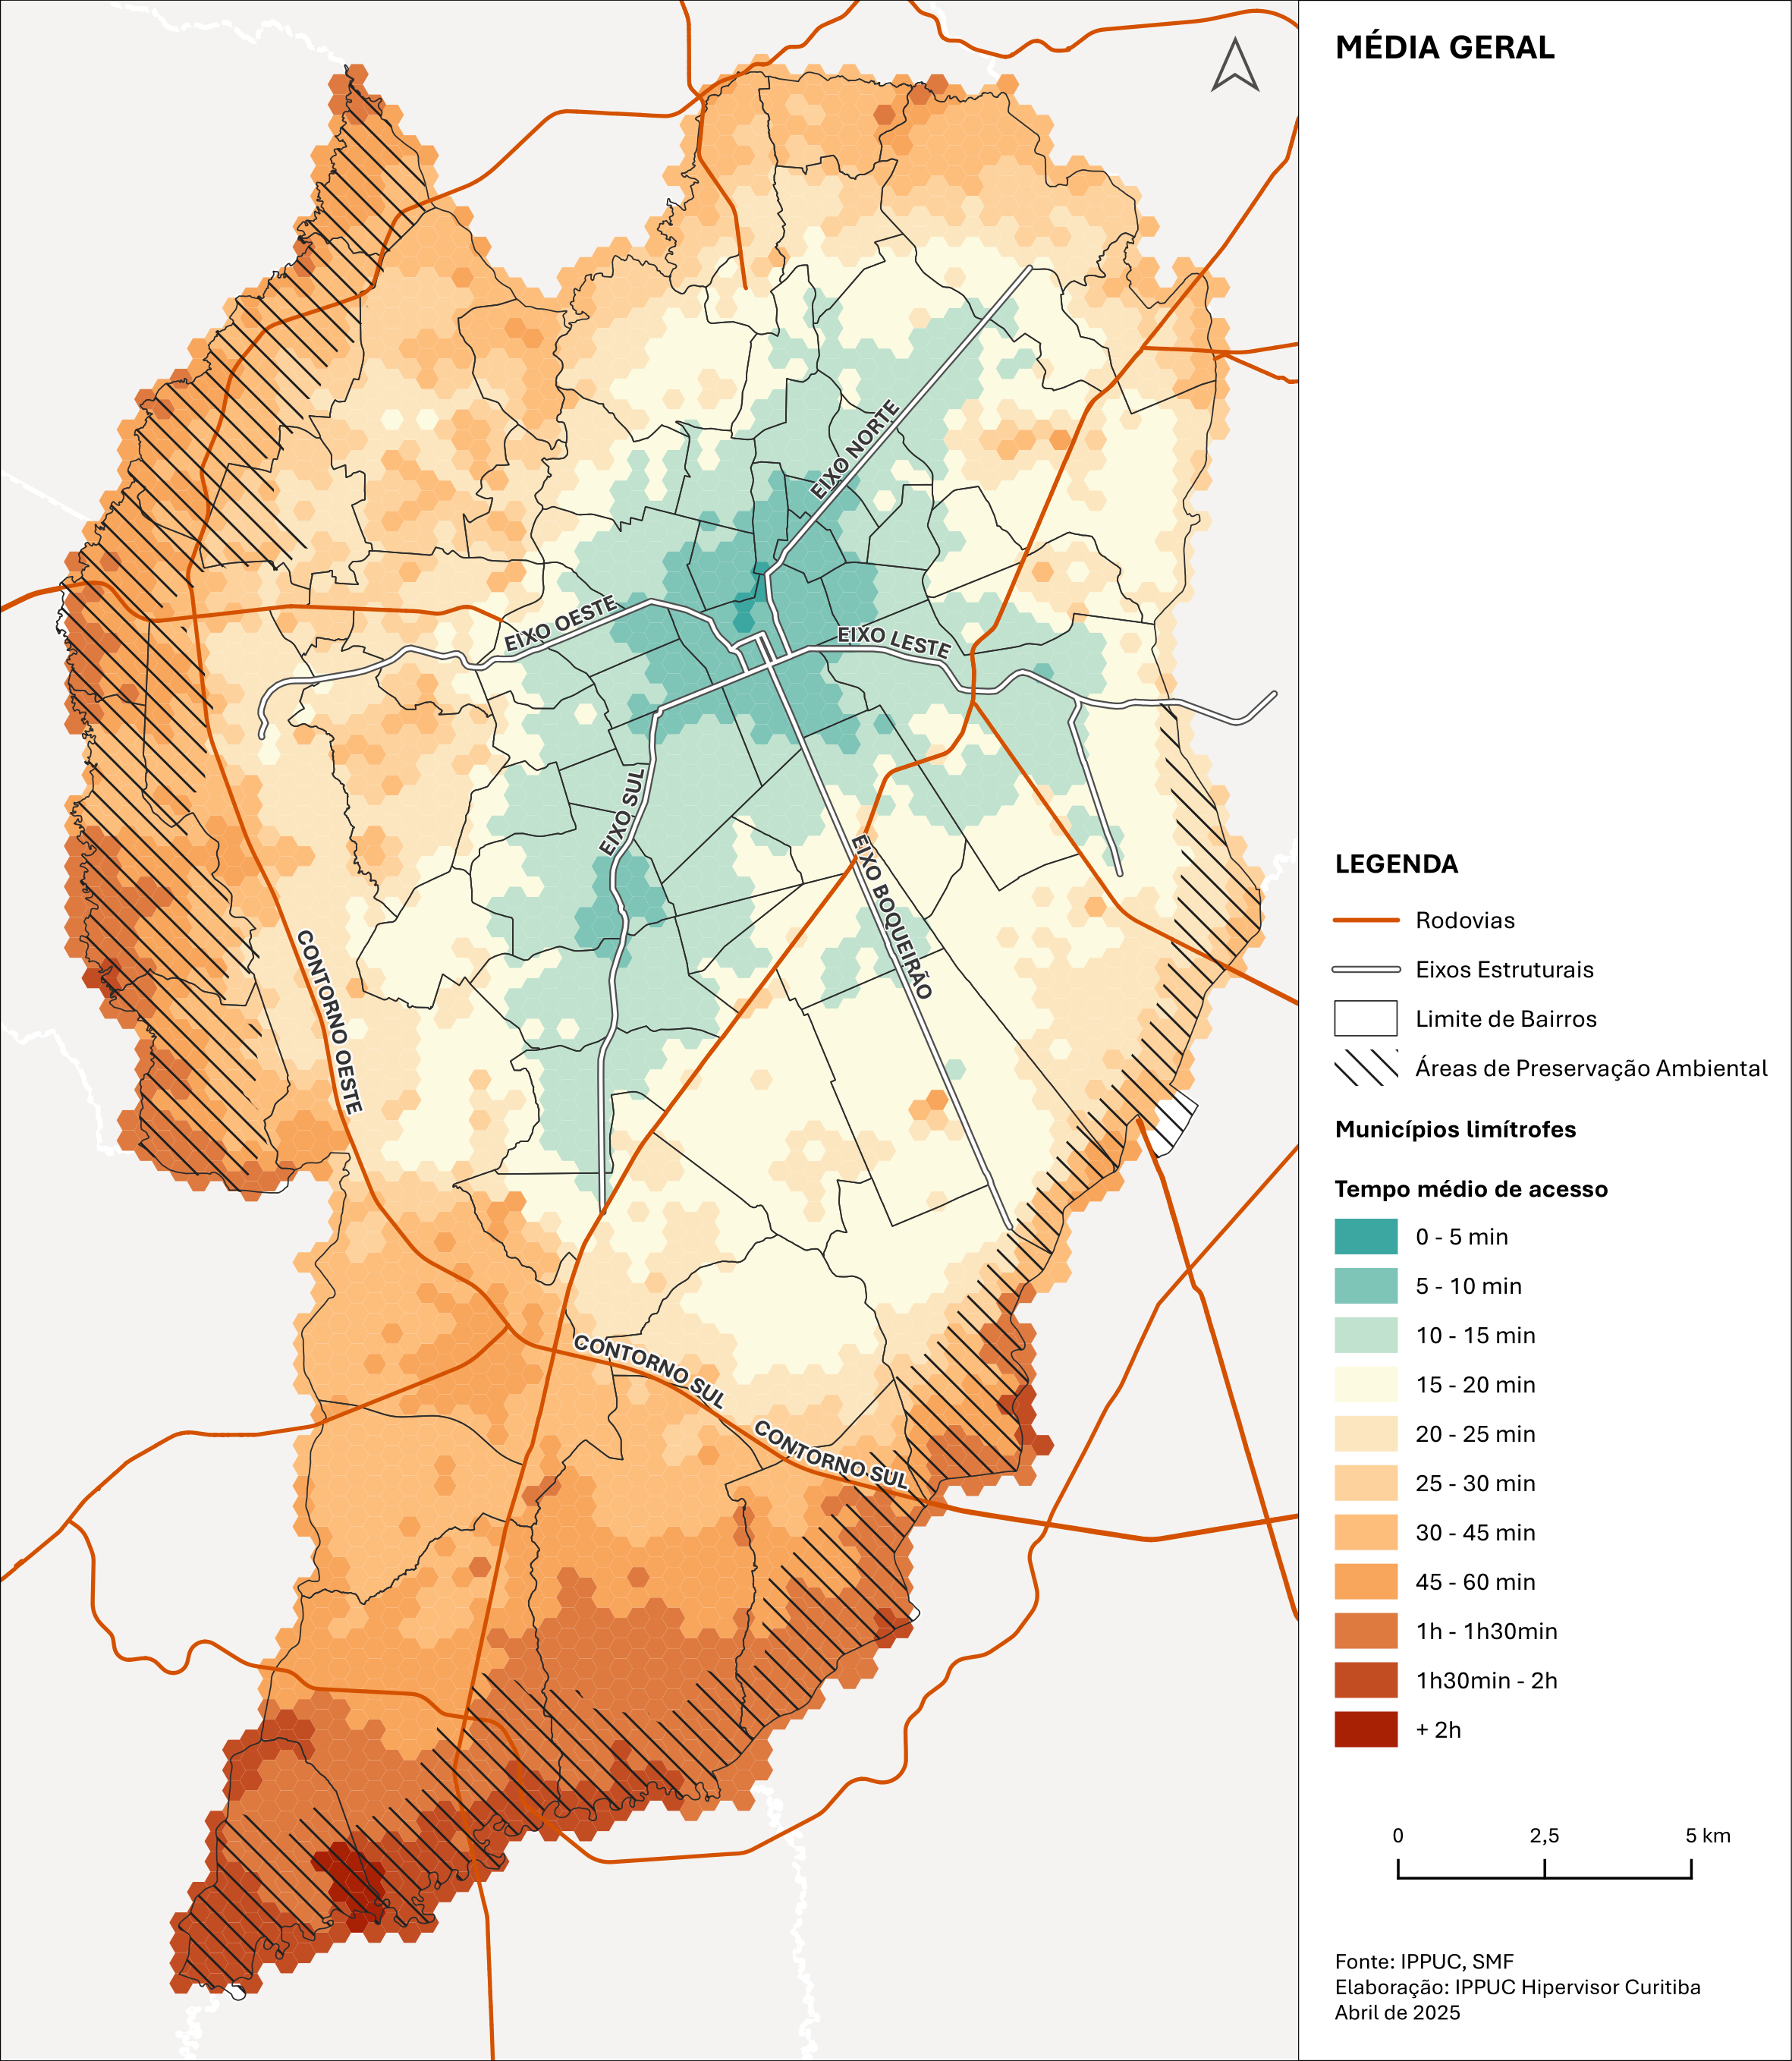
\includegraphics[width=0.6\textwidth]{figs/tempo_acesso.png} % Ou .svg/.eps
  \caption{Tempos de Acesso Intraurbano (Ippuc).}
  \label{fig:access_time}
\end{figure}

A segunda fonte de dados utilizada consiste nos dados do \ac{idhm}\footnote{Disponível em: \url{http://www.atlasbrasil.org.br/acervo/biblioteca}} da Região Metropolitana de Curitiba publicados pelo Atlas do Desenvolvimento Humano no Brasil do \ac{ipea}. Estes dados foram integrados a malha hexagonal de tempos de acesso do \ac{ippuc} seguindo o critério de maior sobreposição espacial, atribuindo a cada hexágono o valor da região censitária com maior intersecção de área. Nestes dados estão presentes variáveis socioeconômicas, como por exemplo: renda, escolaridade, setor produtivo do trabalho, acesso a serviços de saneamento, mortalidade, entre outros.

\subsection{Seleção de Variáveis}

Após o processamento das duas fontes de dados, realizou-se uma seleção de variáveis partindo de um conjunto de 292 fatores, sendo 60 relacionados a tempos de acesso a pé (geral e por categorias). Esta etapa consistiu na eliminação de variáveis multicolineares. Aquelas com correlação de Pearson absoluto superior a 0,9 foram removidas, mantendo-se apenas uma representante de cada par altamente correlacionado. 

\subsection{Modelagem}

A partir das variáveis selecionadas, foi então ajustado um modelo de regressão \ac{ols} com o tempo de acesso como variável resposta. A finalidade da regressão foi compreender a influência das variáveis socioeconômicas nos tempos médios de acesso intraurbano. Também foi realizado o teste Durbin-Watson para validar a não autocorrelação entre os resíduos do modelo. Todo esse processo compôs o Experimento 1 da pesquisa, com resultados descritos na Seção \ref{sec:results}.

Além do modelo de regressão ajustado, realizou-se uma análise de clusterização. Como etapa preparatória, foi conduzida a redução de dimensionalidade usando \ac{pca} com as variáveis padronizadas via Escore-Z. Esta etapa visou a remoção de redundâncias nas variáveis de entrada e a redução de ruídos. Aqui, a variável tempo de acesso foi incluída antes do processamento. O objetivo da clusterização foi segmentar a área urbana em grupos com perfis heterogêneos, onde cada cluster apresentasse diferenças marcantes no tempo médio de acesso e nas características socioeconômicas. O algoritmo utilizado foi o \textit{KMeans} e a escolha do número de clusters foi feita através do método do cotovelo, analisando-se a inércia para k entre 2 e 10. Esta etapa de investigação foi denominada como Experimento 2.